\documentclass[]{article}


\usepackage[margin=1cm,includehead,landscape]{geometry}
\usepackage{fancyhdr}
\usepackage{multicol}
\usepackage{graphicx}
\pagestyle{fancy}

\fancyhead[CO]{AdvElDes - Sébastien Deriaz}
\fancyhead[LE,RO]{}



\begin{document}
\begin{multicols}{3}
\section{Circuits}
\subsection{Amplificateurs opérationnels}
\subsubsection{Single supply, non inverting}
\begin{center}
\includegraphics[width=0.7\columnwidth,page=3]{../KiCad/resume-crop.pdf}
\end{center}
\begin{enumerate}
\item Fonctionne en DC
\item Tension amplifiée autour de $U_{ref}$
\end{enumerate}
$$G=\frac{R_b}{R_a}$$
\subsubsection{Single supply, inverting}
\begin{center}
\includegraphics[width=0.7\columnwidth,page=4]{../KiCad/resume-crop.pdf}
\end{center}
La tension d'entrée est autour de 0 et la tension de sortie est autour de $U_{ref}$
$$G=-\frac{R_1}{R_2}$$
Graph ici...
\subsubsection{Single supply, differential}
\begin{center}
\includegraphics[width=0.7\columnwidth,page=5]{../KiCad/resume-crop.pdf}
\end{center}
$$G=2\frac{R_b}{R_a}$$


\end{multicols}





\end{document}